
%% This file represents a sample second chapter of the main body of the dissertation
%%
%%**********************************************************************
%% Legal Notice:
%% This code is offered as-is without any warranty either
%% expressed or implied; without even the implied warranty of
%% MERCHANTABILITY or FITNESS FOR A PARTICULAR PURPOSE!
%% User assumes all risk.
%% In no event shall any contributor to this code be liable for any damages
%% or losses, including, but not limited to, incidental, consequential, or
%% any other damages, resulting from the use or misuse of any information
%% contained here.
%%**********************************************************************
%%
%% $Id: chapterTwo.tex,v 1.4 2006/08/24 21:12:59 Owner Exp $
%%


% A first, optional argument in [ ] is the title as displayed in the table of contents
% The second argument is the title as displayed here.  Use \\ as appropriate in
%   this title to get desired line breaks
\chapter[Background and Methodology]{Background and Methodology}

\section{Intel Optane DC Persistent Memory}

Persistent memory, also known as Non-volatile Memory (NVM), is a new addition to the memory/storage hierarchy shown in Figure 2 that fills the performance/capacity gap between DRAM and storage by combining traits of both worlds. Like DRAM, persistent memory comes in the form of Dual In-line Memory Modules (DIMMs) that reside on the memory bus. Therefore, applications can access persistent memory like they do with traditional DRAM, eliminating the need to page blocks of data back and forth between memory and storage. However, unlike DRAM DIMMs, persistent memory DIMMs offer greater capacity and can retain data when the system is shutdown or loses power. Thus, persistent memory can dramatically increase system performance and enable a fundamental change in computing architecture.

Intel Optane DC Persistent Memory Module (PMM) is the first commercially available persistent memory technology. This technology comes in DIMM form factor and embeds capacities up to 512GiB. Intel Cascade Lake processors are the first CPUs to support Intel Optane PMM. Like traditional DRAM, the Optane DIMM sits on the memory bus and connects to the processor's integrated memory controller (iMC). Figure 1 shows a typical system configuration of a hybrid node with DRAM and PMM. A user can have up to one Intel Optane DIMM per channel and up to six on a single socket providing capacities up to 3TiB per socket. Thus, an 8-socket system could access up to 24TB of persistent memory.

To ensure persistence, Intel Optane PMM sits within Intel’s asynchronous DRAM refresh (ADR) domain. Intel’s ADR domain ensures that CPU stores that reach the ADR domain will survive a power failure. The iMC maintains read and write pending queues (RPQs and WPQs) for each Optane DIMM and the ADR domain includes WPQs. Once the data reaches the WPQs, the ADR domain ensures that the iMC will flush the updates to persistent memory media on power failure.

The iMC communicates with the Optane DIMM using the DDR-T protocol in cache line access granularity (64B) (Figure 2). The memory access to NVDIMM arrive first at an Apache Pass Controller which coordinates access to the Optane Media. Similar to SSDs, the Optane DIMM perforsms address translation for wear-leveling and bad block management. Thus, it keeps an address indirection table (AIT) for this translation. 

The actual access to storage media occurs after address translation. Intel Optane DIMM physical media access granularity is 256 bytes. Thus, the Controller translates smaller requests into largest 256-byte accesses, causing write amplification as small stores become read-modify-write operations. The controller has a small write-combining buffer to merge adjacent writes.

Intel Optane PMem can operate in two modes: memory and App Direct. Memory mode uses Optane PMem as a large capacity main memory without persistence. DRAM is not visible to the users, and instead it serves as a cache for Optane PMem that is transparently managed by the operating system. In App Direct mode, Optane PMem DIMMs appear as independent, non-volatile storage devices. This allows Optane PMem to be used as a byte-addressable persistent memory that is mapped into the system physical address space and directly accessible by applications [].

% \section{Persistent Memory Development Kit}
% The Persistent Memory Development Kit (PMDK) is a collection of open-source libraries and tools that simplify managing and accessing persistent memory devices. Tuned for both Linux and Windows operating systems, these libraries build on the dax feature described on the SNIA NVM programming specification. The diagram on figure 5 describes the collection of libraries provided by PMDK. Although PMDK’s core libraries provide C APIs, higher level libraries such as pmemkv provide support for other programming systems.

\section{Serverless Computing}

Serverless computing is a cloud computing execution mode that enables developers to deploy their code without provisioning or managing server infrastructure. The term “serverless” is misleading, as servers are still being used by cloud providers to run the code for developers. However, instead of requesting and managing resources, developers simply provide their code, and the cloud providers handle the servers on behalf of their customers. Cloud providers are responsible for provisioning resources, scaling, fault tolerance, monitoring, security patches, and so on. Finally, developers simply pay by the execution time and resources used on their code invocations.

Function-as-a-service (FaaS) is the core compute engine for serverless computing. It was first introduced on 2015 by AWS Lambda, and since then, other commercial and open-source offerings have appeared, i.e., Google Cloud Functions, Azure Functions, Apache OpenWhisk, and others. With FaaS, a developer implements the application logic as stateless functions in a high-level language, such as Java, Python, C, C++, and so on. The code is then packaged together with its dependencies and submitted to the serverless platform. Finally, the developer associates an event to each function, i.e., HTTP requests, file uploads, and more. Once a trigger is fired, the cloud provider executes the code associated with that trigger.

\section{Reinforcement Learning}

Reinforcement Learning (RL) is a subfield of machine learning concerned with learning optimal decision-making policies through interactions with an environment \cite{sutton2018reinforcement}. The fundamental concept underlying RL is the notion of an agent, which takes actions in an environment and receives feedback in the form of rewards, indicating the quality of its decisions. The agent's objective is to learn a policy that maximizes cumulative rewards over time. Moreover, the agent is not provided with explicit instructions on which actions to take; instead, it must discover the actions that lead to the highest rewards by trying them.

\begin{figure}[ht]
    \centering
    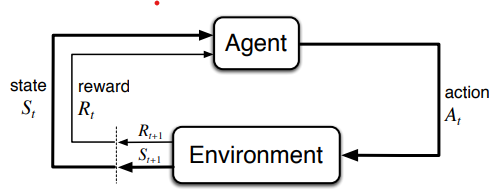
\includegraphics[scale=1]{images/rl-workflow.png}
    \caption{RL Workflow}
    \label{fig:sutton_rl_workflow}
\end{figure}

Figure \ref{fig:sutton_rl_workflow} presents a schematic representation of a standard reinforcement learning scenario. In discrete time steps, the agent perceives the current state $s_t$ from the set of all possible states $S$. It then selects an action $a_t$ from the available actions $A(s_t)$ in the current state. The environment transitions to a new state $s_{t+1}$, and the agent receives a reward $r_t$ associated with the transition $(s_t, a_t, s_{t+1})$.

The agent's behavior is governed by its policy, which maps perceived states to actions. The ultimate aim is to learn an optimal or near-optimal policy that maximizes the cumulative reward. 


\subsubsection*{Q-Learning}

One of the foundational algorithms in RL is Q-Learning, introduced by Watkins in 1989 \cite{watkins1989learning}. The algorithm belongs to the class of model-free RL algorithms, meaning it learns directly from experience without requiring a model of the environment dynamics \cite{russel2020ai}.

At the core of Q-Learning is the Q-value function, denoted as $Q(s, a)$, which represents the expected cumulative reward the agent will receive by taking action $a$ in state $s$ and following an optimal policy thereafter. The objective of Q-Learning is to iteratively update the Q-values based on observed transitions and rewards, eventually converging to the optimal Q-values that maximize long-term rewards.

The Q-Learning algorithm proceeds as follows: the agent interacts with the environment by selecting actions based on its current estimate of the Q-values. Upon taking an action, the agent observes the resulting reward and the next state. It then updates the Q-value of the previous state-action pair using the observed reward and the estimated value of the next state.

The Q-value update rule in Q-Learning is based on the Bellman equation, which expresses the relationship between the Q-values of successive states \cite{russel2020ai}:

\[
Q(s, a) \leftarrow (1 - \alpha) \cdot Q(s, a) + \alpha \cdot \left( r + \gamma \cdot \max_{a'} Q(s', a') \right)
\]

Here, $\alpha$ is the learning rate, determining the extent to which new information overrides the old one, and $\gamma$ is the discount factor, representing the importance of future rewards relative to immediate rewards. The term $r + \gamma \cdot \max_{a'} Q(s', a')$ is known as the temporal-difference (TD) target, combining the immediate reward $r$ with the discounted maximum Q-value of the next state $s'$ \cite{russel2020ai}.

% Q-Learning, a model-free reinforcement learning algorithm, is employed by the agent to determine the best action given the current state. The agent evaluates action quality using a quality-function (Q-function) $Q(s, a)$, representing the expected total discounted reward if the agent selects action $a$ in state $s$ and acts optimally thereafter. 

% One of the foundational algorithms in RL is Q-Learning, introduced by Watkins in 1989 \cite{watkins1989learning}. Q-Learning is a model-free algorithm that learns the value of taking an action in a particular state, known as the Q-value, and iteratively refines these values through experience. The Q-value represents the expected cumulative reward the agent will receive by taking an action in a given state and following an optimal policy thereafter.

% The Q-Learning algorithm (illustrated in Figure \ref{algo:q_learning}) involves iterative updates to the Q-function. At each step, the agent selects an action, observes the reward and new state, and then applies one-step Q-learning. The update is governed by the Q-learning formula, where the learning rate ($\alpha$) determines the extent to which new information overrides old data. This learned Q-function approximates the optimal Q-function, irrespective of the policy being followed.

\subsubsection{Linear Regression Models in Reinforcement Learning}

One of the key advantages of Q-Learning is its simplicity and ease of implementation. It requires only a table to store the Q-values, making it computationally efficient for small state and action spaces. However, Q-Learning faces challenges in environments with large state spaces, as maintaining a lookup table becomes infeasible due to memory and computational constraints.

Function approximation is a fundamental technique in reinforcement learning (RL) aimed at approximating the Q-Value function when dealing with large state or action spaces where tabular representations become impractical \cite{russel2020ai}. This approach allows RL agents to generalize from observed states to unseen states, facilitating decision-making in unexplored regions of the state space.

In the context of RL, linear regression models are commonly used for function approximation \cite{sutton2018reinforcement}.  These models approximate the Q-value function by leveraging a weighted linear combination of features, with each feature capturing a distinct aspect of the state space. Employing gradient-descent methods, notably stochastic gradient descent, enables iterative refinement of the parameters governing the linear function, aimed at minimizing a predefined loss function. This iterative optimization process empowers the model to progressively enhance its predictive accuracy and capture intricate patterns within the state-action space.

Hyperparameter tuning is a critical aspect of training linear regression models in RL \cite{bergstra2012random}. Hyperparameters, such as the learning rate, regularization strength, and feature scaling, significantly impact the performance and convergence of the models. A systematic approach to hyperparameter tuning involves experimenting with different combinations of hyperparameters, evaluating the performance of the trained models on a validation set, and selecting the optimal hyperparameters based on predefined criteria, such as validation error or performance metrics \cite{russel2020ai}.

\subsubsection{Exploration-Exploitation Tradeoff}

The exploration-exploitation tradeoff poses a significant challenge in reinforcement learning \cite{sutton2018reinforcement}. The agent must strike a balance between exploring unfamiliar actions to gather information and exploiting known actions for immediate rewards. Finding this balance is crucial for effective learning and task performance, as the agent gradually favors actions with higher expected rewards.

One classic strategy for balancing exploration and exploitation is the epsilon-greedy (e-greedy) algorithm \cite{sutton2018reinforcement}. The e-greedy policy selects the action that maximizes the estimated value with probability $1 - \epsilon$ (exploitation) and selects a random action with probability $\epsilon$ (exploration). This approach ensures that the agent continues to explore the environment while gradually exploiting more rewarding actions as it gains knowledge.

Decayed e-greedy methods aim to strike a balance between exploration and exploitation by gradually reducing the exploration rate $\epsilon$ as the agent gains more experience or as the training progresses \cite{sutton2018reinforcement}. This decay encourages the agent to explore the environment more extensively in the early stages of learning while gradually shifting towards exploitation as it becomes more knowledgeable.

\subsubsection{Reward shaping}

Reward shaping is a technique in reinforcement learning (RL) aimed at accelerating learning by modifying the reward signal provided to the agent. Traditional RL algorithms rely solely on sparse reward signals, which can make learning slow and inefficient, especially in complex environments. Reward shaping addresses this issue by providing additional, shaped rewards that guide the agent towards desirable behaviors. These shaped rewards are designed to provide more informative feedback to the agent, encouraging it to explore the state-action space more effectively. However, reward shaping must be carefully designed to avoid unintended consequences such as overfitting to the shaped rewards or incentivizing undesirable behaviors \cite{russel2020ai}.

% Reinforcement Learning considers a problem of a learning agent that actively learns from its own experience \cite{sutton2018reinforcement}. Such agent interacts with its environment and periodically receives a reward signal. The agent’s goal is to maximize the rewards in the long run. However, the agent is not told which actions to take. Instead, it must discover the actions that yield the highest rewards through trial-and-error.

% \begin{figure}[ht]
%     \centering
%     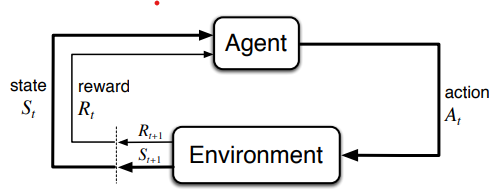
\includegraphics[scale=1]{images/rl-workflow.png}
%     \caption[RL Workflow]{RL Workflow}
%     \label{fig:sutton_rl_workflow}
% \end{figure}

% Figure \ref{fig:sutton_rl_workflow} illustrates a typical reinforcement learning scenario. The agent interacts with the environment in discrete time steps. At each time step t, the agent senses the environment’s current state st E S, where S represent the full set of environment states. It then chooses an action at E A(st), where A(st) represents the set of all actions available in the current state. The environment moves to a new state st+1, and the agent receives a reward rt associated with the transition (st,at,st+1).

% At any given time, the agent’s behavior is defined by a policy. Roughly speaking, a policy is a mapping from perceived states of the environment to actions to be taken when in those states. The agent’s purpose is to learn the optimal, or near-optimal, policy that maximizes total reward it receives in the long run. 
% QLearning
% Q-Learning is a model-free reinforcement learning algorithm, where the agent learns which is the best action to take given the current state. The agent assess the quality of an action by means of a quality-function (Q-function) Q(s,a), denoting the expected total discounted reward if the agent takes action a on state s and acts optimally thereafter. Given the Q-function, the agent’s optimal policy is to choose the action that yields the highest reward.

% Figure 4 illustrates the Q-Learning algorithm. The Q-function can be implemented using a simple lookup table. At each step, the agent selects an action a, and observes the reward r and the new state st+1. Then, the agent applies one-step Q-learning, given by:
% Qlearning formula
% Where 0<alpha<1 is the learning rate and determines to what extent new information overrides the old one. The learned Q-function directly approximates the optimal Q-function, independent of the policy being followed.

% The Q-function can be represented using a simple Q-Table. However, when the state-action space is large, i.e., greater than $10^{6}$ states, keeping a lookup table becomes intractable. To solve this problem, the agent needs to build an approximation of the true Q-function using a function approximator.

% Exploration vs Exploitation tradeoff
% One of the challenges that arises in Reinforcement Learning is the choice between exploiting a familiar action known for a reward and exploring unfamiliar actions for unknown rewards, known as the exploration-exploitation tradeoff. The dilemma is that the agent cannot pursue exploration nor exploitation exclusively without failing the task. Instead, it must find a balance between exploration and exploitation. The agent must try a variety of actions to gather enough information and progressively favor for those that appear to be the best.